\chapter{Resultados}
\label{cap:resultados}

Os resultados a seguir seguem o mesmo protocolo de uso dos modelos discutidos até o momento:

\begin{outline}[enumerate]
    \1 É executado o algoritmo \textbf{auto ARIMA} para obtenção do modelo SARIMAX, com frequência sazonal 24 e todas as variáveis exógenas destacadas na seção \ref{subsec:orig_data} fazendo parte da regressão.
    \1 É executado o algoritmo PSO-ACO SARIMAX.
        \2 Tendo como limite máximo de dimensionalidade para os parâmetros (p,d,q) e (P, D, Q) uma unidade acima do encontrado pelo modelo resultante do \textbf{auto ARIMA}.
        \2 A Sazonalidade é com frequência entre 24 e 48.
        \2 As variáveis exógenas são testadas para saber quais destas de fato ajudam o modelo.
            \3 Precipitação Total (mm)
            \3 Temperatura do Ar (\textdegree{}C)
            \3 Umidade Relativa (\%)
            \3 Velocidade do Vento (m/s)
            \3 Velocidade do Vento em rajada (m/s)
        \2 Se o resultado for pior que o obtido pelo \textbf{auto ARIMA}, este último é mantido. A comparação é feita a partir da métrica AICc.
    \1 O modelo SARIMAX selecionado segue para uso nos modelos híbridos descritos nas subseções \ref{subsec:ag-mlp} e \ref{subsec:ag-mlp-vr}.
        \2 Para todas as séries foi estipulado 80\% de dados para treino, que são utilizados para realizar o treinamento do algoritmo de otimização e hibridização, bem como todas as MLPs e 20\% para teste, que utilizado para avaliação do modelo híbrido final.
\end{outline}

\section{Maceió}

A primeira série temporal escolhida se trata dos últimos 30 dias, entre 12/03/2020 às 21 horas e 11/04/2020 às 20 horas da base para a cidade de Maceió-AL. A Tabela \ref{tab:cap4_comp_autoarima_psoaco} mostra o resultado da comparação entre os algoritmos descritos na seção \ref{subsec:autoarima_psoaco}. 

\begin{table}[htbp]
\caption{Comparação resultados entre \textbf{auto ARIMA} e PSO-ACO.}
\begin{center}
\begin{tabular}{ccccc}
                    & SARIMAX (p,d,q)(P,D,Q,S) & Variáveis Exógenas & AICc & MAPE  \\\hline
\textbf{auto ARIMA} & (1,0,2)(1,0,2,24) & Todas & -1488.858 & \textbf{5.3497} \\\hline
PSO-ACO             & (2,0,0)(1,0,1,24) & Temperatura do Ar & \textbf{-1516.263} & 6.7475 \\\hline
\label{tab:cap4_comp_autoarima_psoaco}
\end{tabular}
\end{center}
\end{table}

Como descrito no início do capítulo, e pelo que foi obtido, optou-se por utilizar a modelagem SARIMAX obtida descrita na segunda linha da Tabela \ref{tab:cap4_comp_autoarima_psoaco}, como entrada para os algoritmos híbridos descritos pela seções \ref{subsec:ag-mlp} e \ref{subsec:ag-mlp-vr}, resultando finalmente nos resultados descritos pela Tabela \ref{tab:cap4_comp_agmlp_agmlpvr}.

\begin{table}[htbp]
\caption{Avaliação do erro entre modelos satelitais, radiação direta normal e métrica proposta.}
\begin{center}
\begin{tabular}{ccccc}
                & MAE & MSE & MAPE \\\hline
SARIMAX         & 0.035221 & 0.002941 & 2.91303 \\\hline
Híbrido AG-MLP  & \textbf{0.024321} & \textbf{0.001857} & 0.90901 \\\hline
Híbrido AG-MLP-VR & 0.02684 & 0.002439 & \textbf{0.530453} \\\hline
\label{tab:cap4_comp_agmlp_agmlpvr}
\end{tabular}
\end{center}
\end{table}

Um resultado gráfico pode ser observado na Figura \ref{fig:cap4_maceio_3_days_hibrids} em que se mostra as 3 formas de modelagem e o seu resultado sobre as últimas 72 horas de dados.

\begin{figure}[!htbp]
    \centering
    \caption{Últimas 72 horas do resultado utilizando algoritmo AG-MLP descrito na seção \ref{subsec:ag-mlp}.}
    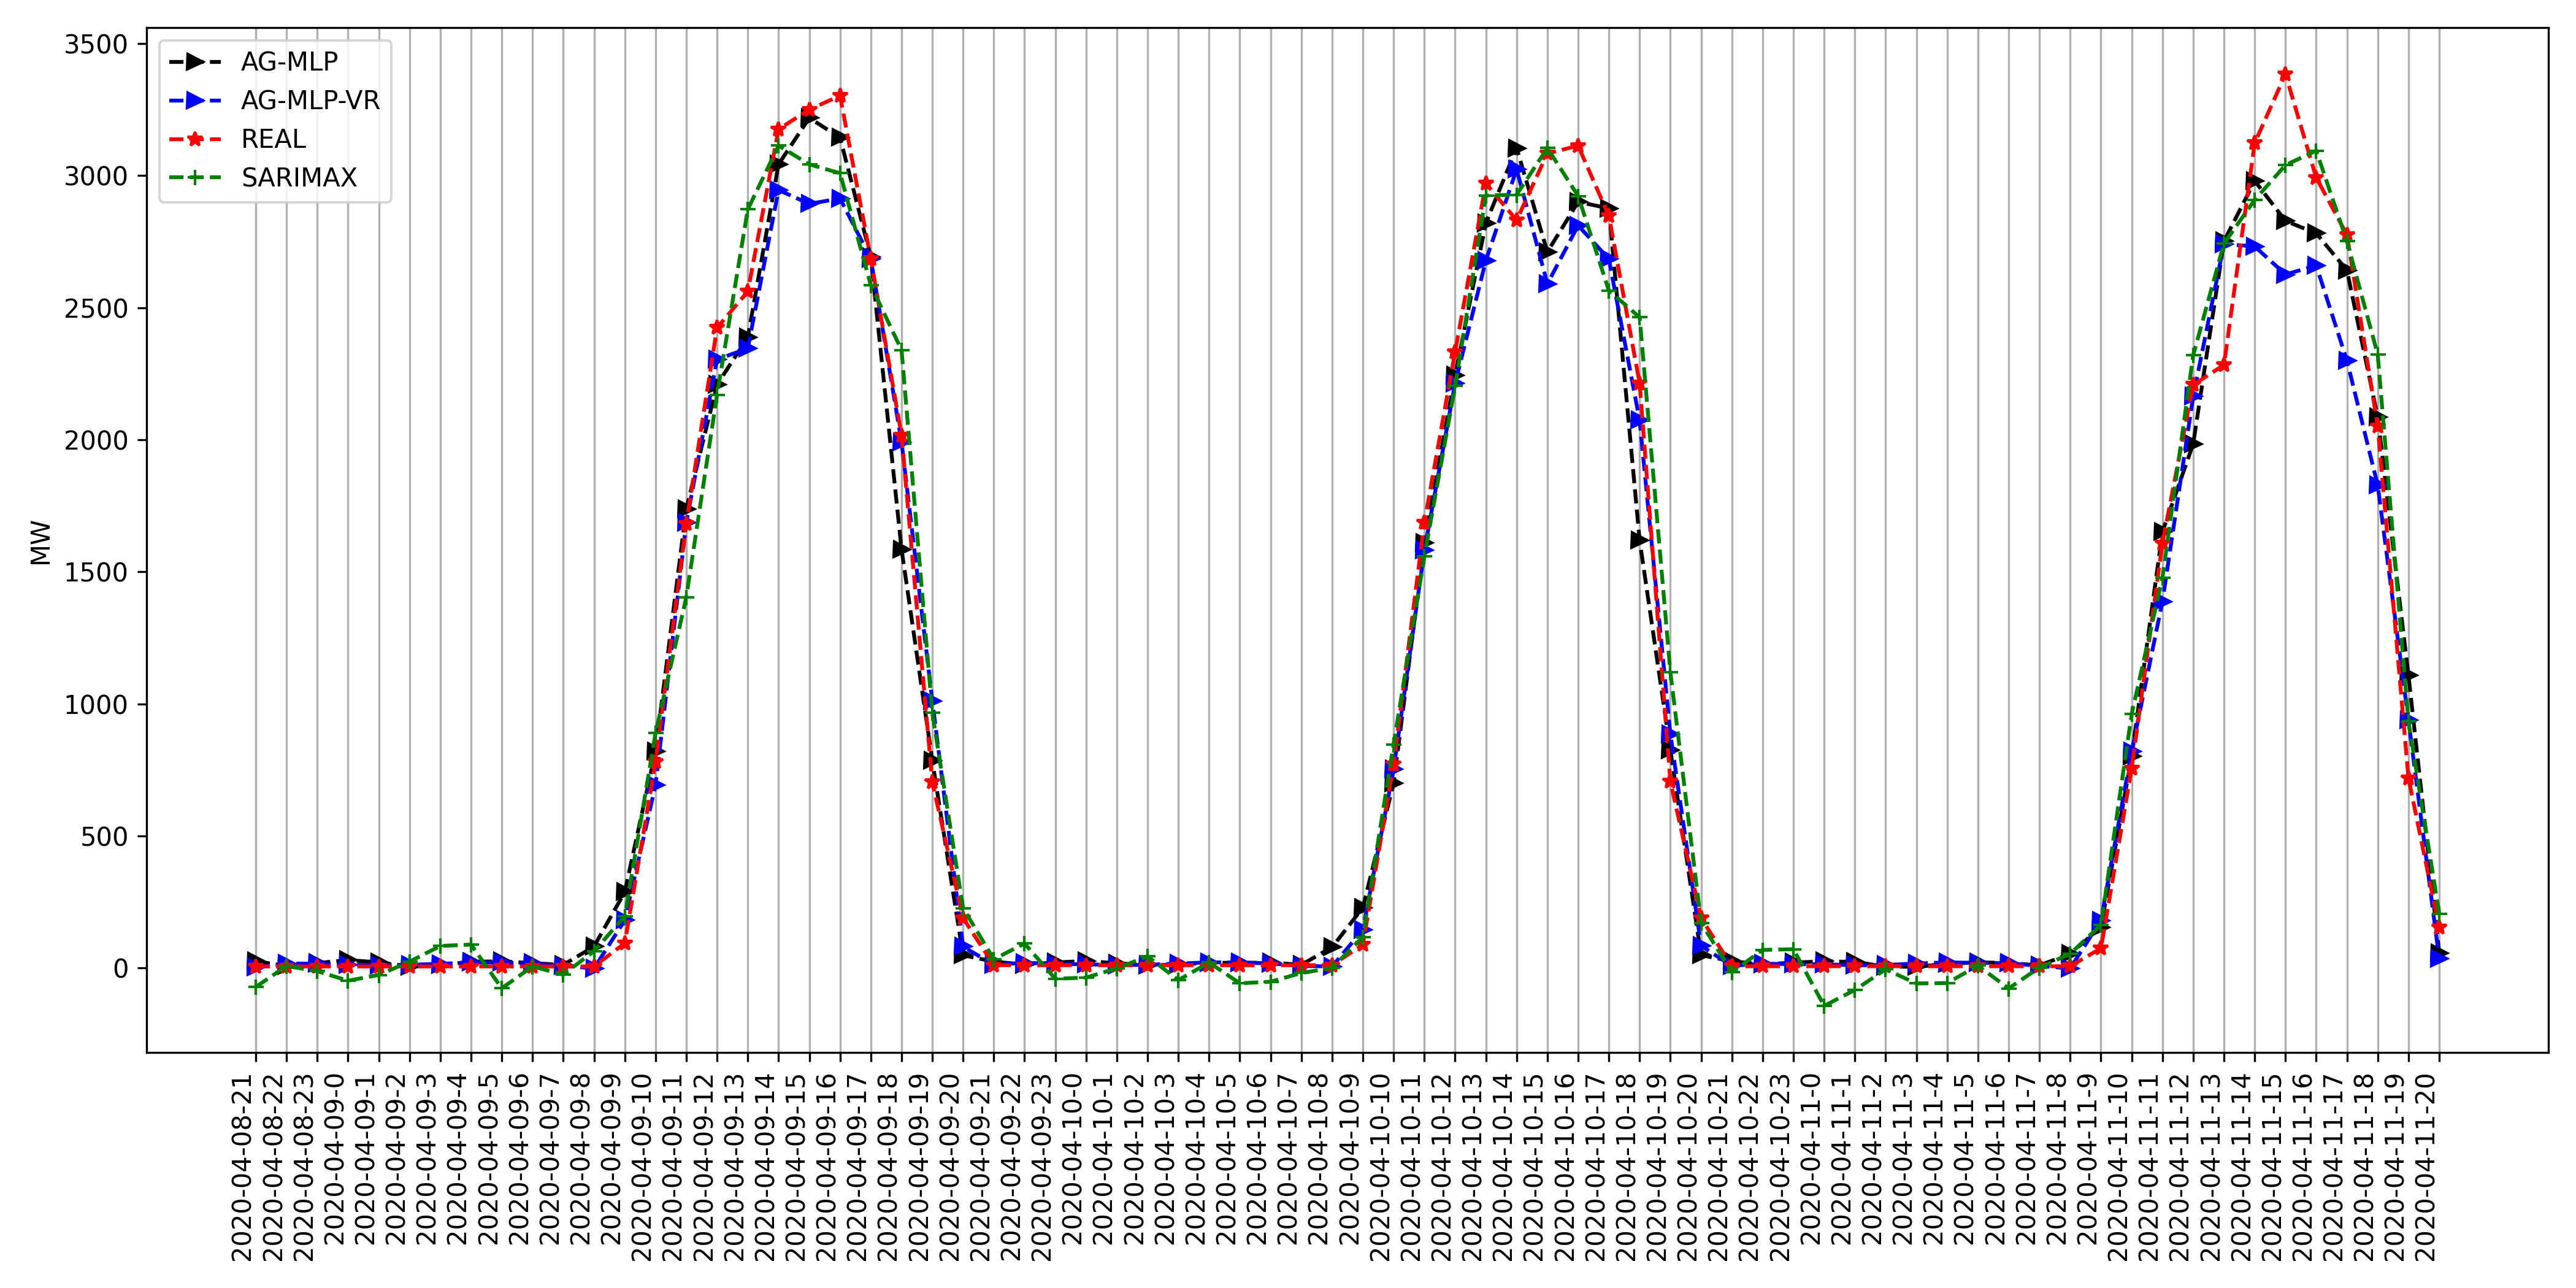
\includegraphics[width=\textwidth]{Figuras/cap4/comparison_hibrids.png}
    \source{Autor.}
    \label{fig:cap4_maceio_3_days_hibrids}
\end{figure}

\section{Florianópolis}

